\newtheorem{definition}{Definition}
\newtheorem{theorem}{Theorem}
\section{Introduction}
The area of this study is non-linear dynamics. The evolution of many systems can be defined as the iteration of a non-linear function. The focus in this report is on functions operating from and to the set of complex numbers, $f:\mathbb{C}\to \mathbb{C}$. Of particular interest are the fixed points $x_0$ where $f(x_0)=x_0$. Mainly, fixed points will be found for the Newton iteration function, which is an efficient root-finding method. The behaviour of the Newton method will be explored in different regions of the complex plane. Where does it converge or  diverge? What fixed points are there? In which areas do chaos occur? 
%Many equations are difficult to solve, but a tool to solve them is Newton's iteration method. 
%
\subsection{Basic Concepts}
In this section the concepts of iteration, orbit and fixed point will be defined. First of all, iteration is something repeating over and over. 
\begin{definition}
For an iterated function application we introduce the notation
\begin{eqnarray*}
f^0(x)     &= &x\\
f^{n+1} &= &f\circ f^n
\end{eqnarray*}
\end{definition}
\noindent 
For example $f^1(x)=f(x)$ and $f^2(x)=f(f(x))$.

Starting from any number (called seed), we can use iteration to define a sequence of numbers, and we call this sequence an orbit.
\begin{definition}
An orbit of $x$ under $f$ is an infinite sequence starting with $x$, where each new term has an extra iteration of $f$. The orbit $O_f(x)$ is \[O_f(x)=[x, f(x), f^2(x),\ldots].\]
\end{definition}
\noindent
For example, the orbit of the seed $1$, under the function $g(x)=2x$ is $[1,2,4,8,16,\ldots]$. This orbit tends to infinity. But using the seed $0$, the orbit is constant: $[0,0,\ldots]$

In general, an orbit can tend to infinity (as in the first example), be a fixed point (as in the second example) or be periodic. An example of a periodic orbit is the orbit of the seed $0$ under the function $h(x)=1-x$. The orbit, $[0,1,0,1,0,1,\ldots]$, consists of $0$ and $1$ repeating over again, so the period is $2$. Consequently, a fixed point, has a period of $1$. This means that the orbit of $x$ consists of the same point over again: $[x, x, x,...]$. 

These fixed points might seem quite dull, but actually they are rather interesting. There are three categories of fixed points, attracting, neutral and repelling. For an attracting fixed point, the x-values nearby move toward the attracting fixed point when repeatedly iterated. For a repelling fixed point the x-values nearby move away when repeatedly iterated. For a neutral fixed point, the values neither move towards nor from the point. The formal definition is as following.
\begin{comment}
\hrule
\textbf{TODO:}
\begin{enumerate}
    \item{Kolla upp absolutbelopp komplext i bok}
    %\item{Är fraktaler relevant?}
\end{enumerate}
\hrule
\end{comment}

\begin{definition}
Given a fixed point $x$ under $f$, $x$ is attracting if $\abs{f'(x)}<1$, neutral if $\abs{f'(x)}=1$ and repelling if $\abs{f'(x)}>1$.
\end{definition}
\noindent
For example, consider the function $g(x)=x$. It consists only of neutral fixed points since $\abs{f'(x)}=1$. Next, consider $h(x)=\sqrt{x}$. It has a fixed point at $1$. If we take the orbits of two close points $1.1$ and $0.9$ we get $[1.10,1.05,1.02,1.01,...]$ and $[0.90,0.95,0.97,0.99,...]$. We see that both points seem to approach 1, it seems to be attracting. It can be shown to be attracting using the formal definition that since $h'(x)$ is equal to $\frac{1}{2\sqrt{x}}$ we have that
\[h'(1)=\frac{1}{2\sqrt{1}}=\frac{1}{2\cdot1}=\frac{1}{2}<1\]
%
Now, as we have studied fixed points, let us move onward to critical points. 
\begin{definition}
A point $x$ of $f(x)$ is critical, if the derivative, $f'(x)$, is equal to $0$. %s.95
\end{definition}
This means that the point can be a maximum or minimum point, or it can be an inflexion point. In the case where it is a maximum or a minimum point, the second derivative of $f$ gives us information on which of these points it is. Unfortunately it does not give us information if it is an inflexion point.

%
\subsection{Newton's Iteration Function and Conjugacy}
\begin{comment}
\hrule
\textbf{TODO:}
\begin{enumerate}
    \item{Jag vet att det finns ett samband mellan Newtons iteration method och conjugacy men har inte riktigt kunnat binda ihop dem än.}
    \item{Jag har inte heller introducerat innebörden av att funktioner är conjugate.}
\end{enumerate}
\hrule
\end{comment}
The Newton iteration function $N_f$ is a method to find the roots for a given function $f$ with an initial guess, $x$. The expression for the function is 
\[N_f(x)=x-\frac{f(x)}{f'(x)}.\]
The Newton iteration function, has orbits and fixed points such as any other function. The attracting fixed points of $N_f$, are of great interest, since they are in one-to-one correspondence with roots of $f$. This is described in the theorem below. \parencite{yau}
 %\parencite{bae}
\begin{theorem}
Given a function $f$, $x_0$ is a root to $f$ if and only if $x_0$ is a fixed point to the Newton iterated function of $N_f$. Additionally, such a point is always attracting.
\end{theorem}
This means that if you have found an attracting fixed point of $N_f$ it is a root to $f$. As a consequence, there may be other fixed points to $N_f$, that are neutral or repelling, but these fixed points are not roots of $f$.  
Now let us move on to conjugacy in functions.

\begin{definition}
We say that $f:X\to X$ and $g:Y\to Y$ are conjugate if there is a homeomorphism $h:X\to Y$ such that $h\circ f=g\circ h$.
\end{definition}
Does $h\circ f=g\circ h$ hold for all iterations of $f$ and $g$? 
\begin{theorem}
Show $h\circ f^n=g^n\circ h$ for all $n\in\mathbb{N}$. 
\end{theorem}
\begin{proof}

I apply proof by induction. The base case is when the iteration is 0.
\[h\circ f^0=h=g^0\circ h\]
Assume that $h\circ f^m=g^m\circ h$ for all $m=0,1,2,...n$. We now want to show that $h\circ f^{n+1}=g^{n+1}\circ h$. So we start with the left hand side of the equation and show that it is equal to the right hand side. First the left hand side, $h\circ f^{n+1}$, can be rewritten as $h\circ f^n\circ f$. Now we use the assumption $h\circ f^n$ is equal to $g^n\circ h$. Then we can rewrite the left hand side further as $g^n\circ h\circ f$. Now we use that $f$ and $g$ are conjugate, that $h\circ f=g\circ h$. We have that
\[g^n\circ h\circ f=g^n\circ g\circ h.\]
Finally we simplify this to $g^{n+1}\circ h$ which is the right hand side of the equation.
\end{proof}
We have showed that the homeomorpism holds for all iterations of $f$ and $g$. By showing this we have showed that the orbit for one function $f$ is equal to the orbit of another function $g$ if they are conjugate.
%
\begin{comment}
\subsection{Complex Plane and the Mandelbrot Set}
Complex numbers are the foundation of the fractals in the Mandelbrot set. Complex numbers are part real and part imaginary. The imaginary unit $i^2$ is equal to $-1$. 

By iterating the function $F_c(z)=z^2+c$, where c is a complex number, fractals occur, causing the Mandelbrot set. The algorithm depends on iteration, and connected sets. \parencite{projecteuclid}
\end{comment}
%
\newpage
\section{Project}
Consider the family of functions $f_{a}(z)=(z^2-1)(z^2+a)$ for different values of $a$. The purpose of this project is to design a program to plot the set of $a$-values for which the critical point $c_+(a)$ of $N_{f_a}$ does not tend to one of the four roots of $f_{a}$. \parencite{bae}

%(Then design a program to plot the orbit diagram for the Newton iteration function $N_{f_a}$ using $c_+(a)$ of $N_{f_a}$ as the seed for each orbit.) 

%Focus on the vicinity of $a=0.16$, Mandelbrot set?

%
\subsection{Important points for $f_a$ and $N_{f_a}$}
First lets find some of the relevant points related to $f_a$ and $N_{f_a}$. What are the 4 roots to $f_a$? Either $(z^2-1)$ or $(z^2+a)$ is equal to $0$. Then we have $z=\pm1$ and $z=\pm\sqrt{a}i$. These four roots will be the attracting fixed points of $N_{f_a}$, so they will be clearly visible. Additionally, in the vicinity of these four points the Newton iteration function will probably be effective.

Now let's explore $N_{f_a}$- The Newton iteration function for $f_a$ is 
\[N_{f_{a}}(z)=z-\frac{f_a(z)}{f_a'(z)}=z-\frac{(z^2-1)(z^2+a)}{((z^2-1)(z^2+a))'}.\]
This can be expanded to
\[z-\frac{z^4-z^2+az^2-a}{4z^3+2az-2z}\]
which can be rewritten as
\[\frac{4z^4+2az^2-2z^2}{4z^3+2az-2z}-\frac{z^4-z^2+az^2-a}{4z^3+2az-2z}.\]
Lastly this can be simplified as
\[\frac{3z^4+az^2-z^2+a}{4z^3+2az-2z}=\frac{3z^4+z^2(a-1)+a}{4z^3+2z(a-1)}=\frac{3z^4+z^2(a-1)+a}{4z(z^2+\frac{(a-1)}{2})}.\]
This is undefined if the denominator $4z(z^2+\frac{(a-1)}{2})$ is equal to $0$. We have the roots $z=0$ and $z=\pm\sqrt{\frac{1-a}{2}}$. Therefore I state the hypothesis that the graph will approach infinity if $z$ approaches $0$ or $\pm\sqrt{\frac{1-a}{2}}$. 

We can calculate the critical points to $N_{f_a}$. They are when  
\[N_{f_a}'=0\]
Using the quotient rule for derivation we have
\[N_{f_a}'=\frac{(3z^4+z^2(a-1)+a)'\cdot(4z(z^2+\frac{(a-1)}{2})-(3z^4+z^2(a-1)+a)\cdot(4z(z^2+\frac{(a-1)}{2})'}{(4z(z^2+\frac{(a-1)}{2})^{2}}.\]
Simplifying this gives us
\[\frac{(12z^3+2az-2z)\cdot(4z(z^2+\frac{(a-1)}{2})-(3z^4+z^2(a-1)+a)\cdot(12z^2+2a-2)}{(4z(z^2+\frac{(a-1)}{2})^{2}}\]

%
\newpage
\section{Algorithm}
An algorithm was designed to plot a bitmap of how many iterations of the Newton iteration function are needed for various functions $f_a$ in different points in the complex plane. This was done for different values of $a$.
%
\newpage
\section{Results}
The algorithm was done for different values of $a$. In Figure \ref{results} two bitmaps show how many iterations are needed for $N_{f_a}$.

\begin{figure}[h!]
	\centering
	\begin{subfigure}[b]{0.4\textwidth}
		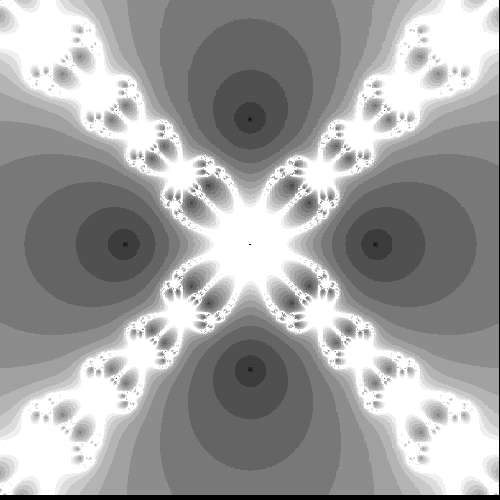
\includegraphics[width=\textwidth]{a=1.png}
		\caption{The graph of the Newton iteration function $N_{f_{a}}(z)$ when $a=1$.}
		\label{a1}
	\end{subfigure}
	\hspace{5pt} %lite kul med extra mellanrum?
	\begin{subfigure}[b]{0.4\textwidth}
		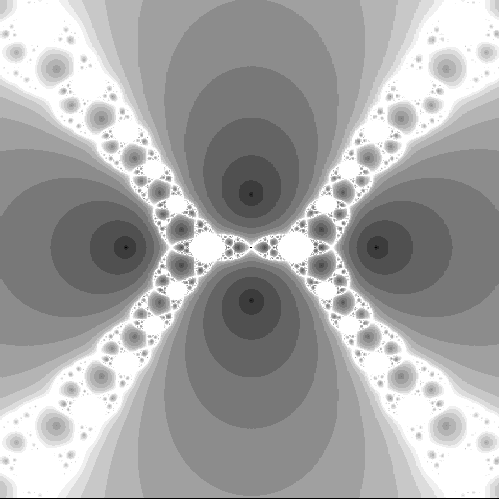
\includegraphics[width=\textwidth]{a=018.png}
		\caption{The graph of the Newton iteration function $N_{f_{a}}(z)$ when $a=0.18$.}
		\label{a018}
	\end{subfigure}
	\caption{The graphs for $N_{f_{a}}(z)$ between $z=-2-2i$ and $z=2+2i$ for different values of $a$.}
	\label{results}
\end{figure}

Here we can see that the four roots of $f_a(z)$ are black. But something chaotic has occured on the four diagonal lines.

%
\newpage
\section{Discussion}
%
\addcontentsline{toc}{section}{Acknowledgment}
\section*{Acknowledgement}
\begin{comment}
I would like to thank Jenny Homann, my supervisor, for help in this project. I am also very thankful for computer science professor Patrik Jansson for help with programming in Haskell. %I am also thankful for friends and family who have taken the time to read and give feedback on this paper.
\end{comment}
\addcontentsline{toc}{section}{References}


























\begin{comment}
Now, let us define the concept fractal. The concept of fractals are not entirely necessary for this project.
\begin{definition}
A fractal is a subset of $\mathbb{R}^n$ which is self-similar and which fractal dimension exceeds its topological dimension.
\end{definition}

Now what does this mean? First of all, fractals are self-similar. Subsections of the fractal is the same as the whole. This leads to that fractals are not merely one or two dimensional, since they are infinite. In particular fractal objects do not have integer dimension, they rather have a fractal dimension, which can be a fraction. \parencite{tufillaro}.
\end{comment}

\begin{comment}
\hrule
\textbf{TODO:}
\begin{enumerate}
    \item{Förklara the orbit diagram}
\end{enumerate}
\hrule
\end{comment}

%(I defined the Newton's iteration function, but calculated the derivate for hand. Maybe later I can define the derivative.)
%
\begin{comment}
\subsection{Chaos}
Chaos is a nonlinear deterministic process which appears to be random. In fact it is fairly predictable. \parencite{economics} A fractal does not have a single scale of length, chaos generates complex fluctuations that do not have a single or characteristic scale of time \parencite{lipsitz}. \parencite{yale}
\end{comment}
\begin{comment}
The Newton iteration function has an attracting cycle with period 2 at the critical points
\[c_\pm(a)=\sqrt{\frac{1-a}{6}}.\] 
It may be attracted to the fixed points of $N(x)$ or it may not, does $c(a)$ converge to the roots of $f(x)$ or does it not. \parencite{bae}
We find that N is an odd function, since $N(-x)=-N(x)$.
Vid critical points ska derivatan av fa vara lika med 0:
2z(2z²+a-1)->z=0 eller 2z²=1-a->z=+-sqrt(1-a/2)
Andraderivatan kan ge vilken karaktär punkten har. Den är 12z²+2a-2. 
Tre fall. Om z=0 då 2a-2. Då om a=1 så är det jobbigt. Om a>1 då positiv andra derivata. 
Om z=sqrt(1-a/2), vilket nog är c+. Vad är då andraderivatan på olika a? 6*(1-a)+2*(a-1)=6*(1-a)-2*(1-a)=4*(1-a). Andraderivatan är positiv för a<1. Då har punkten en positiv krökning, alltså lokalt minimum. För z=0.66 om a=0.16. Då har xvärdet=-0.3363 
Korsar i +-1. Varje a som är mindre än 1 så har den ett minimi runt z=0. Om a=0 då rot i z=0. När fungerar newton iterationen som lösning och när fungerar den inte. FInns lurigt maaximum nära 0 som ändå inte är 0. 
\end{comment}
\begin{comment}
\begin{code}
map h.iterate f x=
map h [x, f x, f^2 x,...]=
[h x, g.h x, g.h.f x]=
[h x, g.h x, g.g.h x]=
[h x, g.h x, g^2 h x]=
iterate g.h
\end{code}
\end{comment}